%%%
%
% $Autor: Wings $
% $Datum: 2021-05-14 $
% $Pfad: GitLab/MLEdgeComputer $
% $Dateiname: L298N
% $Version: 4620 $
%
% !TeX spellcheck = de_DE/GB
% !TeX program = pdflatex
% !BIB program = biber/bibtex
% !TeX encoding = utf8
%
%%%



\chapter{Entwicklerboard - Motorsteuerung DEBO MotoDriver2 L298N}

Um die zwei verwendeten Motoren ansteuern zu können, wird die Erweiterungsplatine DEBO MotoDriver2 L298N benutzt. Diese erlaubt die Steuerung und Versorgung von bis zu zwei Gleichstrommotoren. Die Motoren können mit Spannungen zwischen 5V und 35V angetrieben werden. Der verwendete Chipsatz ist L298N. Es wird auf dem Logiklevel von 5V gearbeitet. Die Ausgangsleistung beträgt 25W bei einem maximalen Treiberstrom von bis zu 2A. Die Abmaße der Platine sind 43mm $\times$ 43mm $\times$ 27mm. In der folgenden Abbildung \ref{fig:L298N} ist die Erweiterungsplatine zu sehen.


\begin{figure}
    \centering
    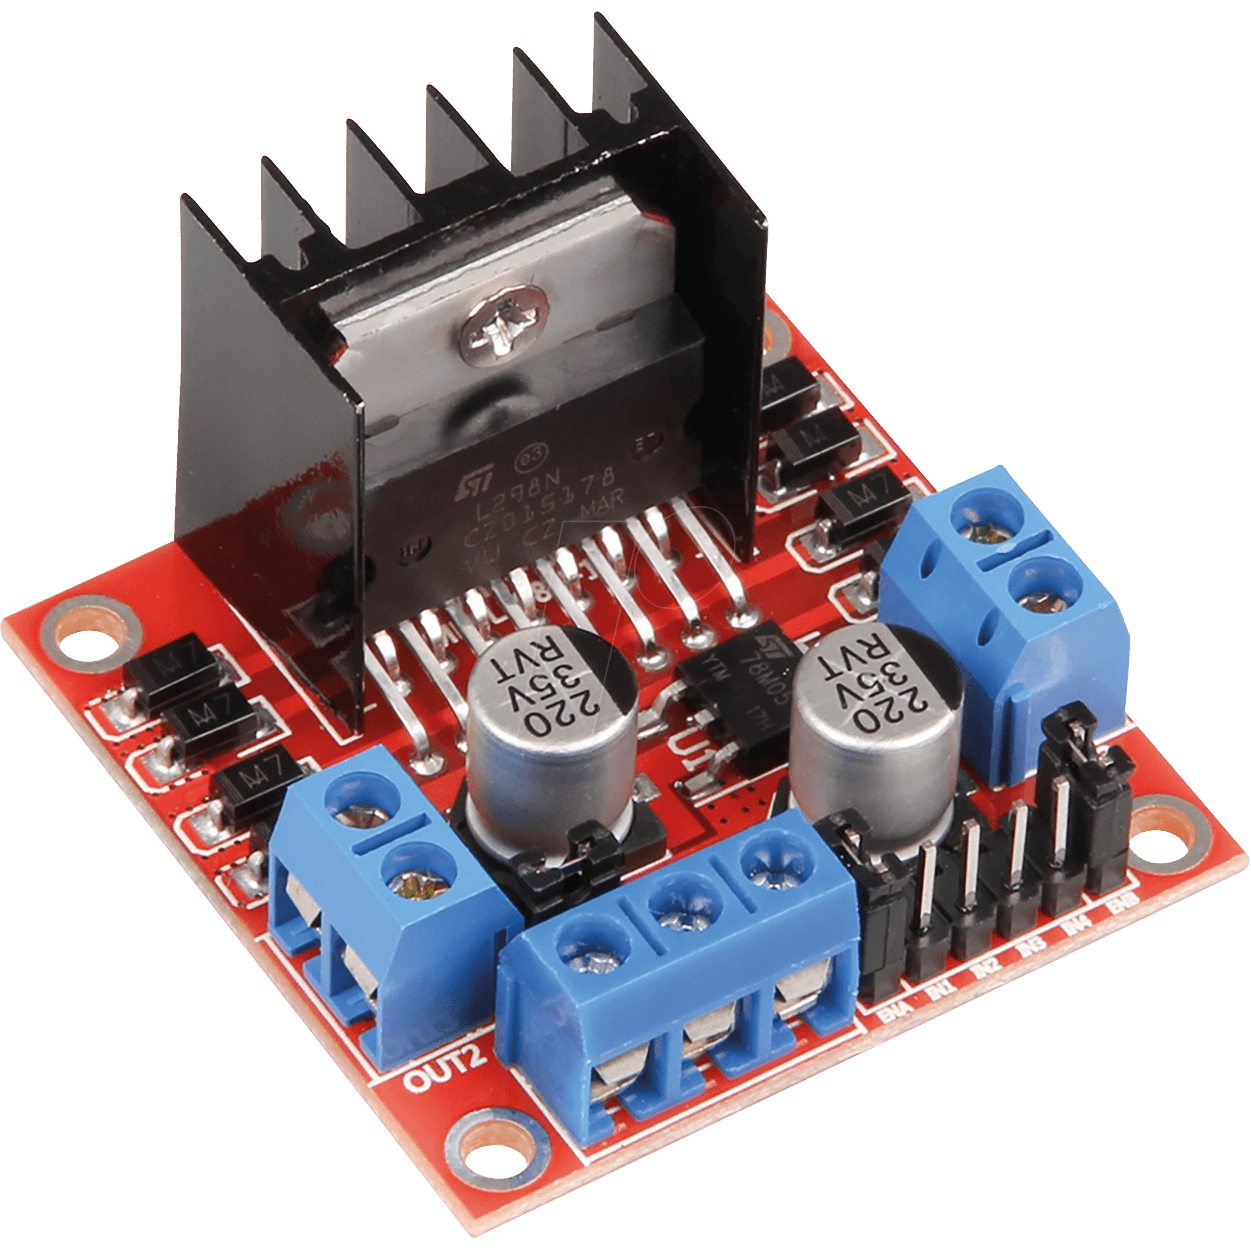
\includegraphics [width=70mm] {L298N/L298N}
    \caption{Motorsteuerung DEBO MotoDriver2 L298N}
    \label{fig:L298N}
\end{figure}

In der folgenden Abbildung \ref{fig:driverpin} sind die Pins des Treibers beschriftet und in der Tabelle \ref{tab:driver_pin} ist die Pinbelegung dargestellt. \cite{Simac:2019b}

\begin{figure}
    \centering
    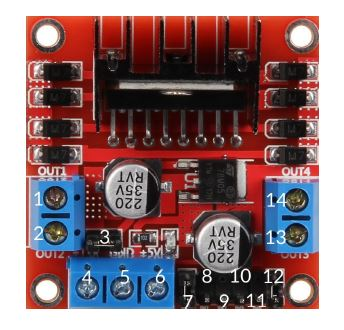
\includegraphics [width=70mm] {L298N/AnschlussDriver}
    \caption{Treiber mit Beschriftung}
    \label{fig:driverpin}
\end{figure}
\begin{table}[h]
    \centering
    \begin{tabular}{|c|c|}
        \hline
        \textbf{PIN}           & \textbf{Belegung}                          \\ \hline
        1                          & DC Motor 1 / Stepper Motor +       \\ \hline
        2                          & DC Motor 1 / Stepper Motor GND      \\ \hline
        3                          & 12V Jumper       \\ \hline
        4                          & Stromversorgung +       \\ \hline
        5                          & Stromversorgung GND      \\ \hline
        6                          & 5V Ausgang (wenn Jumper 3 gesetzt)     \\ \hline
        7                          & DC Motor 1 Jumper       \\ \hline
        8                          & Input 1       \\ \hline
        9                          & Input 2      \\ \hline
        10                          & Input 3       \\ \hline
        11                         & Input 4       \\ \hline
        12                          & DC Motor 2 Jumper      \\ \hline
        13                          & DC Motor 2 / Stepper Motor +       \\ \hline
        14                          & DC Motor 2 / Stepper Motor GND       \\ \hline
    \end{tabular}
    \caption{Pinbelegung des Treibers}
    \label{tab:driver_pin}
\end{table}

